% This is samplepaper.tex, a sample chapter demonstrating the
% LLNCS macro package for Springer Computer Science proceedings;
% Version 2.20 of 2017/10/04
%
\documentclass[runningheads]{llncs}
%
\usepackage{graphicx}
\usepackage{hyperref}
\hypersetup{hypertex=true,
colorlinks=true,
linkcolor=blue,
anchorcolor=blue,
citecolor=blue}
\usepackage[ruled]{algorithm2e}
\usepackage{booktabs} 
\usepackage{multirow}
\usepackage{array}
\usepackage{diagbox}
% Used for displaying a sample figure. If possible, figure files should
% be included in EPS format.
%
% If you use the hyperref package, please uncomment the following line
% to display URLs in blue roman font according to Springer's eBook style:
% \renewcommand\UrlFont{\color{blue}\rmfamily}

\begin{document}
%
\title{Contribution Title\thanks{Supported by organization x.}}
%
%\titlerunning{Abbreviated paper title}
% If the paper title is too long for the running head, you can set
% an abbreviated paper title here
%
\author{First Author\inst{1}\orcidID{0000-1111-2222-3333} \and
Second Author\inst{2,3}\orcidID{1111-2222-3333-4444} \and
Third Author\inst{3}\orcidID{2222--3333-4444-5555}}
%
\authorrunning{F. Author et al.}
% First names are abbreviated in the running head.
% If there are more than two authors, 'et al.' is used.
%
\institute{Princeton University, Princeton NJ 08544, USA \and
Springer Heidelberg, Tiergartenstr. 17, 69121 Heidelberg, Germany
\email{lncs@springer.com}\\
\url{http://www.springer.com/gp/computer-science/lncs} \and
ABC Institute, Rupert-Karls-University Heidelberg, Heidelberg, Germany\\
\email{\{abc,lncs\}@uni-heidelberg.de}}
%
\maketitle              % typeset the header of the contribution
%
\begin{abstract}
The abstract should briefly summarize the contents of the paper in
15--250 words.

\keywords{First keyword  \and Second keyword \and Another keyword.}
\end{abstract}
%
%
%
\section{First Section}
\subsection{A Subsection Sample}
Please note that the first paragraph of a section or subsection is
not indented. The first paragraph that follows a table, figure,
equation etc. does not need an indent, either.

Subsequent paragraphs, however, are indented.

\subsubsection{Sample Heading (Third Level)} Only two levels of
headings should be numbered. Lower level headings remain unnumbered;
they are formatted as run-in headings.

\paragraph{Sample Heading (Fourth Level)}
The contribution should contain no more than four levels of
headings. Table~\ref{tab1} gives a summary of all heading levels.



%%%%%%%%%%%%%%%%%%%%%%%%%%%%%%%%%%%%%%%%%%%%%%%%%%%%%%%%%%%%%%%%%%%%%%%%%%%%%%%%%%%%%%%%%%%%%%%%%%%%%%

\section{Group decomposition based on 4D approximation}\label{Sec3}
We select the better group among the points through the approximation hypervolume of each pair of points in the same layer. Exactly, we will select the pair of points which has the abstract zone with smaller hypervolume. Because the value of the hypervolume exactly is a iterval, so the smaller hypervolume of a pair of points means the over-approximation of the hypervolume is smaller than under-approximation of others or the hypervolume has a smaller over-approximation than others which has overlapping with the interval of the hypervolume. At first, we assume that all of the hypervolume and volume mentioned following are convex and all of the situations dicussed following under the $k=2$.
\\We will introduct how to expand convex volume calculation formular from three dimension to four dimension, how to obtain the under- and over- approximation of four-dimensional hypervolume in order.

\subsection{Expand convex volume calculation formula to four dimensiton}

\begin{theorem}\label{T1}
Making a three-dimensional prismatic cone as the base volume which volume is V, like the base area of a three-dimensional prismatic cone, integrating the volume of the three-dimensional prismatic cone alone the forth dimension, we will get a hypervolume of four-dimensional prismatic cone $V^{(4)}$, which equals to

\begin{equation}\label{A}
V^{(4)}=\frac{1}{4}V^{(3)}h^{(4)}
\end{equation} 

In equation \ref{A}, $h^{(4)}$ is the value of the forth dimension, like the ‘height’ in three-dimensional situation and $V^{(3)}$ is the volume as the base of the four-dimensional prismatic cone. Before deriving \ref{A}, we will first review the derivation of volume for a three-dimensonal prismatic cone.
\end{theorem}

\begin{proof}
The main idea is to consider a three-dimensional prismatic cone as a pile of cubes~\cite{ref_book1}. For example, in Fig.~\ref{FigR1_1}, ABCD is a convex polygon on the yOz plane and its area is S. The three-dimensional prismatic cone is consisted of several cubes with base areas similar to the base area ABCD. That means if we use a plane paralleling to ABCD to intercept the prismatic cone J-ABCD, we will get a intersection area ${A}'{B}'{C}'{D}'$which is similar to ABCD. As a result, there exists a similarity between the areas of ${A}'{B}'{C}'{D}$(the area is defined as ${S}'$) and S:

\begin{equation}\label{A1}
{S}'=\frac{S\cdot x^{2}}{h^{2}} 
\end{equation}

x is the distance between ${A}'{B}'{C}'{D}'$ and ABCD , h is the whole height of the three-dimensional prismatic cone J-ABCD.

\begin{figure}
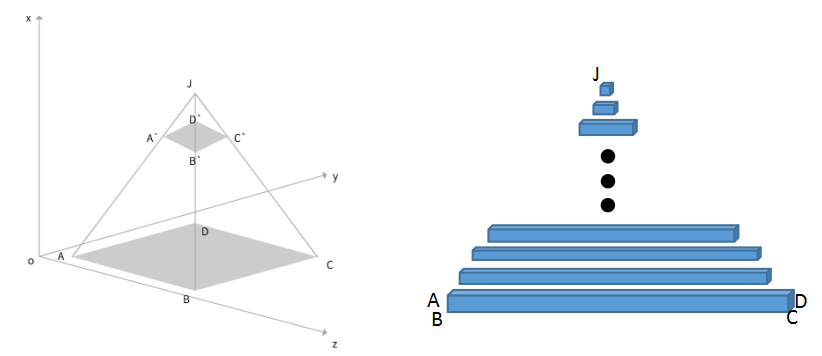
\includegraphics[width=\textwidth]{Fig/FigR1_1.png}
\caption{The right picture of Fig.~\ref{FigR1_1} means if we use a plane paralleling to ABCD to intercept the prismatic cone J-ABCD, we will get a intersection area ${A}'{B}'{C}'{D}'$which is similar to ABCD. The right one means that the three-dimensional prismatic cone is consisted of several cubes with base areas similar to the base area ABCD.} \label{FigR1_1}
\end{figure}

For every cube as component of the J-ABCD, its volume definded as $V_{i}$, i=1,2,...,n.According to the similarity theorem: 

\begin{equation}\label{A2}
V_{i}=\lim \limits_{n \to \infty}\frac{h}{n}\cdot \frac{S\cdot x_{i}^{2}}{h^{2}}
\end{equation}

As mentioned before, a three-dimensonal prismatic cone can be considered as a pile of cubes, so the whole volume of J-ABCD can be expressed as:

\begin{equation}\label{A3}
V=\lim \limits_{n \to \infty}\sum_{i=1}^{n}\frac{h}{n}\cdot \frac{S\cdot x_{i}^{2}}{h^{2}}
\end{equation}

For $\frac{h}{n}\in \left ( 0,1\right ]$ and $x_{i}\in \left [ 0,h\right ]$, equation \ref{A3} and the conception of definite integration can be expressed as:

\begin{equation}\label{A4}
V=\int_{0}^{h}\frac{S\cdot x^{2}}{h^{2}}dx = \frac{1}{3}Sh
\end{equation}

equation \ref{A4} is the general volume formula of a three-dimensional prismatic cone.
Now we have reviewed the expansion from two-dimensional area to three-dimensional volume, it's time to expand from three-dimensional volume to four-dimensional prismatic cone.
Comparing to the situation from two-dimensional area to three-dimensional volume,a four-dimensional prismatic cone as a pile of hypercubes(assume that there are n such hypercubes, marked as $H_{i}$, i=1,2,...,n), and if we use a three-dimensional space paralleling to the base of the four-dimensional prismatic cone to intercept the four-dimensional hypervolum, the intersection volume(which is three-dimensional) is similar to the base three-dimensional volume~\cite{ref_url1}, like Fig.~\ref{FigR1_2}.

\begin{figure}
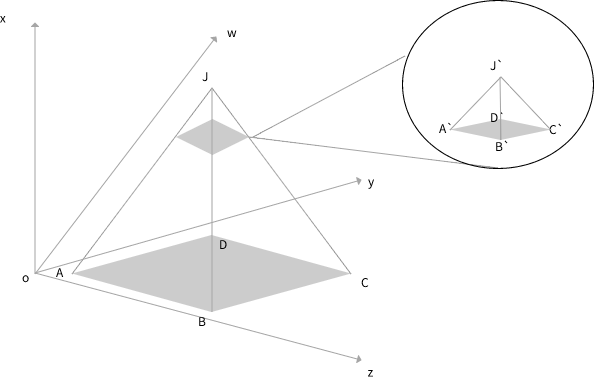
\includegraphics[width=\textwidth]{Fig/FigR1_2.png}
\caption{The picture of Fig.~\ref{FigR1_2} means if we use a three-dimensional space paralleling to the base of the four-dimensional prismatic cone to intercept the four-dimensional hypervolum JABCD, the intersection volume ${J}'-{A}'{B}'{C}'{D}'$(which is three-dimensional) is similar to the base three-dimensional volume} \label{FigR1_2}
\end{figure}

If we mark the volume of base three-dimension volume as $V^{(3)}$, the value of the forth dimension as $h^{(4)}$, the intersection volumes as  $V_{i}^{(3)}$, i=1,2,...,n, like the derivation of equation \ref{A1} according to the similarity theorem:
\begin{equation}\label{B}
V_{i}^{(3)}=\frac{V^{(3)}\cdot x_{i}^{(4) 3}}{h^{(4) 3}} 
\end{equation} 
In equation \ref{B}, $x_{i}^{(4)}$ is the distence from the base volume to each of the hypercubes $H_{i}$. As same as the derivation above, the hypervolum of each four-dimensional hypercubes can be expressed as:

\begin{equation}\label{B1}
V_{i}^{(4)}=\lim \limits_{n \to \infty}\frac{h^{(4)}}{n}\cdot \frac{V^{(3)}\cdot x_{i}^{(4) 3}}{h^{(4)3}}, i=1,2,...,n
\end{equation}

So the whole hypervolume defined as $V_{(4)}$ can be expressed as:

\begin{equation}\label{B2}
V^{(4)}=\lim \limits_{n \to \infty}\sum_{i=1}^{n}\frac{h^{(4)}}{n}\cdot \frac{V^{(3)}\cdot x_{i}^{(4) 3}}{h^{(4) 3}}
\end{equation}
Because of $\frac{h^{(4)}}{n}\in \left ( 0,1\right )$
\begin{equation}\label{B3}
V^{(4)}=\int_{0}^{h^{(4)}}\frac{V^{(3)}\cdot x^{(4) 3}}{h^{(4) 3}}dx^{(4)} = \frac{1}{4}V^{(3)}h^{(4)}
\end{equation}

\end{proof}

%%%%%%%%%%%%%%%%%%%%%%%%%%%%%%%%%%%%%%%%%%%%%%%%%%%%%%%%%%%%%%%%%%%%%%%%%%%%%%%%%%%%%%%%%%%%%%%%%%%%%%

\subsection{Obtain approximations of four-dimensional convex hypervolume}

Because the state-of-the art algorithms for hypervolume calculation are time-consuming, the runtime is more than $O(d^{4})$~\cite{ref_article2}, d is the number of edges in a hypervolume, or preform far from pretty while facing the value of the hypervolume is a interval with perturbation in neuron net although they can get a approximation of the hypervolume more accurate than ours~\cite{ref_article3}. 

\begin{definition}\label{Def1}
Assume that there is a fully connected net N with n pre-activation layers and there are $n_{s}$ neurons(or points) in the s th pre-activation layer of N, $s\in \left \{1,2,...,n\right \}$. Point i and j mean the i th and j th points among the $n_{s}$ points in the s th pre-activation layer of N, $i,j\in \left \{1,2,...,n_{s}\right \},i\neq j$. A point also means a tuple $(x,y)$, x is the output of the point as the pre-activation value to ReLU layer, y means the result of ReLU(x).

When calculating 2-relu, $k=2$, assume that the pre-activation value and ReLU result of point i are $x_{1}$ and $y_{1}$, similarly we have $x_{2}$ and $y_{2}$ of point j. And we start spliting quadrants from $x_{1}$ dimention, as a result, the $y_{2}$ will be the additional forth dimention.

Given the set of three-demensional constraints $C^{(3)}$, $c_{\left ( i,j\right )}^{(3)}\in C^{(3)}$ is defined as three-denmensional constraints generated from point i and j. Given the set of four-demensional constraints $C^{(4)}$, $c_{\left ( i,j\right )}^{(4)}\in C^{(4)}$ is defined as four-denmensional constraints generated from point i and j. Define that $c^{(3)}_{\left ( i,j\right ),\left \{x\leq 0\right \}}$ be the part of $c_{\left ( i,j\right )}^{(3)}$ satisfying the constrain $x\leq 0$ and $x\in \left \{x_{1},x_{2},y_{1}\right \}$. Similarly,  $c^{(3)}_{\left ( i,j\right ),\left \{x\geq 0\right \}}$ be the part of $c_{\left ( i,j\right )}^{(3)}$ satisfying the constrain $x\geq 0$. In addition, define $c_{(i,j),\left \{ c_{\left ( i,j\right )}^{(3)}\wedge c^{y_{2}}\right \}}^{(4)}$ as a $c_{\left ( i,j\right )}^{(4)}$ whose four-dimensional constrains are consisted of $c_{\left ( i,j\right )}^{(3)}\in C^{(3)}$ and a unitary linear constraint $c^{y_{2}}$ about the forth dimension $y_{2}$, we can find that the constrains of $c_{(i,j),\left \{ c_{\left ( i,j\right )}^{(3)}\wedge c^{y_{2}}\right \}}^{(4)}$ equals to the ones of $c_{\left ( i,j\right )}^{(3)}\wedge c^{y_{2}}$.
\\For example,  $c_{\left ( i,j\right ),\left \{ c^{(3)}_{\left ( i,j\right ),\left \{x\leq 0\right \}}\wedge y_{2}=0\right \}}^{(4)}$ means the part of $c_{\left ( i,j\right )}^{(3)}\in C^{(3)}$ satisfying the constrain $x\leq 0$ and a unitary linear constraint $y_{2}=0$ about $y_{2}$ make up a set of four-dimensional constraints $c_{\left ( i,j\right ),\left \{ c^{(3)}_{\left ( i,j\right ),\left \{x\leq 0\right \}}\wedge y_{2}=0\right \}}^{(4)}\in C^{(4)}$.
\end{definition}

\begin{definition}\label{Def2}
According to Def.~\ref{Def1}, we can define volume of the abstract zone of $c_{\left ( i,j\right )}^{(3)}\in C^{(3)}$ as $V_{\left \{c_{(i,j)}^{(3)} \right \}}^{(3)}$, and hypervolume of the abstract zone of $c_{\left ( i,j\right )}^{(4)}\in C^{(4)}$ as  $V_{\left \{c_{(i,j)}^{(4)} \right \}}^{(4)}$ whose upper and  lower approxiations are defined as $V_{\left \{c_{(i,j)}^{(4)} \right \},upper}^{(4)}$ and $V_{\left \{c_{(i,j)}^{(4)} \right \},lower}^{(4)}$ respectively.
\end{definition}

%%%%%%%%%%%%%%%%%%%%%%%%%%%%%%%%%%%%%%%%%%%%%%%%%%%%%%%%%%%%%%%%%%%%%%%%%%%%%%%%%%%%%%%%%%%%%%%%%%%%%%

Now, we have defined some symbols, it is time to get the formula of the four-dimentional approximations. For example, assume that one of the three-dimensional abstract zones generated by PRIMA is a cube, shown by the left picture of Fig.~\ref{fig3}. Then we add the forth dimension $y_{2}$ to expand the three-dimensional abtract zone to a four-dimensional one, the result shown by the middle of Fig.~\ref{fig3}. Finally, the blue part of the right one is the abstrat of 
\par $conv(c_{\left ( i,j\right ),\left \{ c^{(3)}_{\left ( i,j\right ),\left \{x_{2}\geq 0\right \}}\wedge y_{2}=x_{2}\right \}}^{(4)},c_{\left ( i,j\right ),\left \{ c^{(3)}_{\left ( i,j\right ),\left \{x_{2}\leq 0\right \}}\wedge y_{2}=0\right \}}^{(4)})$ which is the final four-dimensional convex hull $c_{(i,j)}^{(4)}$ obtained by PRIMA.
\begin{figure}
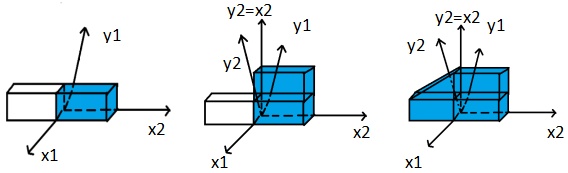
\includegraphics[width=\textwidth]{Fig/FigR2_1.png}
\caption{We assume that the left picture is one of the three-dimensional abstract zones $c^{(3)}_{( i,j)}$ generated by PRIMA, the shape of the abstract zone is a cube, its blue part is the abstract zone of $c^{(3)}_{\left ( i,j\right ),\left \{x_{2}\geq 0\right \}}$.
The blue part of the middle one is the abstract zone of $c_{\left ( i,j\right ),\left \{ c^{(3)}_{\left ( i,j\right ),\left \{x_{2}\geq 0\right \}}\wedge y_{2}=x_{2}\right \}}^{(4)}$. the blue part of the right one is the abstrat of $conv(c_{\left ( i,j\right ),\left \{ c^{(3)}_{\left ( i,j\right ),\left \{x_{2}\geq 0\right \}}\wedge y_{2}=x_{2}\right \}}^{(4)},c_{\left ( i,j\right ),\left \{ c^{(3)}_{\left ( i,j\right ),\left \{x_{2}\leq 0\right \}}\wedge y_{2}=0\right \}}^{(4)})$ which is the final four-dimensional convex hull $c_{(i,j)}^{(4)}$ obtained by PRIMA.} \label{fig3}
\end{figure}

According to the properties of the four-dimensional abstract zone generated by PRIMA, we use $\frac{1}{4}V^{(3)}_{\left \{c^{(3)}_{\left ( i,j\right ),\left \{x_{2}\geq 0\right \}}\right \}}u_{2}$ as the under-approximation of hypervolume and $\frac{1}{4}V^{(3)}_{\left \{c^{(3)}_{( i,j)}\right \}}u_{2}$ as the over-approximation of hypervolume, of which $u_{4}$ is the upper bound of $y_{2}$. Here is a example in Fig.~\ref{fig4} about the under- and over- approximation based on Fig.~\ref{fig3} and we will give the proof about approximation in the following part.

\begin{figure}
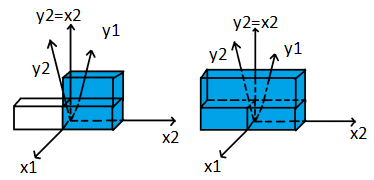
\includegraphics[width=\textwidth]{Fig/FigR2_2.png}
\caption{In the left part of this picture, we directly use the $V^{(3)}_{\left \{c^{(3)}_{\left ( i,j\right ),\left \{x_{2}\geq 0\right \}}\right \}}$ as the base, the upper bound of $x_{2}$, $u_{2}$, as the four-dimensional 'height' to structure the under-approximation $V^{(4)}_{ \left \{ c^{(3)}_{\left ( i,j\right ),\left \{x_{2}\geq 0\right \}}\wedge y_{2}=x_{2}\right \} }$. In the right part of this picture, we use the $V^{(3)}_{\left \{c^{(3)}_{\left ( i,j\right )}\right \}}$ as the base, the upper bound of $x_{2}$, $u_{2}$, as the four-dimensional 'height' to structure the over-approximation $V^{(4)}_{ \left \{ c^{(3)}_{\left ( i,j\right )}\wedge y_{2}=x_{2}\right \} }$} \label{fig4}
\end{figure}

Before giving the proof about approximation, give Theorem~\ref{T2} first as the front theorem for the proof of approximation.

\begin{theorem}\label{T2}
According to the geometric significance and properties of eterminant~\cite{ref_article1} ,the volume of a three-dimensional convex polyhedra can be expressed as a sum of volumes of some three-dimensional prismatic cones, and the hypervolume of a four-dimensional convex polyhedron can be expressed as a sum of hypervolumes of some four-dimensional prismatic cones. The hypervolume of a four-dimensional convex polyhedron can be expressed by a sum of volumes of some three-dimensional prismatic cones.

\begin{proof}
Assume that the hypervolume of a four-dimensional convex pollyhdron is $V^{(4)}$,we have known that $V^{(4)}$ can be expressed as a sum of hypervolumes of several four-dimensional prismatic cones marked as $V^{(4)}_{1},V^{(4)}_{2},...,V^{(4)}_{n}$, the base of each of the $V^{(4)}_{i},i=1,2,...,n$ is marked as $V^{(3)}_{base_{i}}$,i=1,2,...,n. We have known that $V^{(3)}_{base_{i}}$ can be expresses as a sum of volumes of several three-dimensional prismatic cones marked as $V^{(3)}_{i,1},V^{(3)}_{i,2},...,V^{(3)}_{i,n_{i}}$, $n_{i}$ is the number of three-dimensional prismatic cones consisting $V^{(3)}_{base_{i}}$, with the help of Theorem.~\ref{T1}, we can get the relationships between $V^{(4)}$ and $V^{(3)}_{i,j},i=1,2,...,n,j=1,2,...,n_{i}$,$h^{(4)}_{i}$ is the forth dimension 'height' of each of $V^{(4)}_{i}$:

\begin{equation}\label{E}
V^{(4)}=\sum_{i=1}^{n}V^{(4)}_{i}=\sum_{i=1}^{n}\frac{1}{4}h^{(4)}_{i}V^{(3)}_{base_{i}}=\sum_{i=1}^{n}\frac{1}{4}h^{(4)}_{i}\sum_{j=1}^{n_{i}}V^{(3)}_{i,j}
\end{equation}

\end{proof}
\end{theorem}

According to Theorem.\~ref{T2}, we are able to find relationships between three-dimensional convex hull and four-dimensional convex hull in order to obtain the under- and over- approximation mentioned before.

%%%%%%%%%%%%%%%%%%%%%%%%%%%%%%%%%%%%%%%%%%%%%%%%%%%%%%%%%%%%%%%%%%%%%%%%%%%%%%%%%%%%%%%%%%%%%%%%%%%%%%
% lower proof
\begin{proof}
For two selected points i and j, their precise constrains formed by PRIMA is marked as $c_{\left ( i,j\right ),precise}^{(4)}\in C^{(4)}$, so with the help of Def.~\ref{Def1} and Def.~\ref{Def2}, the hypervolume of the abstract zone from $c_{\left ( i,j\right ),precise}^{(4)}$ can be marked as $V^{(4)}_{\left \{c_{\left ( i,j\right ),precise}^{(4)}\right \}}$. There has a equation according to the process of PRIMA or k-ReLU(assume that split about $x_{1}$ firstly so that the $y_{2}$ will be the forth dimention):

\begin{equation}\label{C}
c_{\left ( i,j\right ),precise}^{(4)} = conv(c_{\left ( i,j\right ),\left \{ c^{(3)}_{\left ( i,j\right ),\left \{x_{2}\leq 0\right \}}\wedge y_{2}=0\right \}}^{(4)}, c_{\left ( i,j\right ),\left \{ c^{(3)}_{\left ( i,j\right ),\left \{x_{2}\geq 0\right \}}\wedge y_{2}=x_{2}\right \}}^{(4)})
\end{equation}\\

Previously there has inequality relationships:

\begin{equation}\label{C1}
V^{(4)}_{\left \{c_{\left ( i,j\right ),precise}^{(4)}\right \}} \geq V^{(4)}_{\left \{ c^{(3)}_{\left ( i,j\right ),\left \{x_{2}\geq 0\right \}}\wedge y_{2}=x_{2}\right \}}
\end{equation}

Otherwise, it will have contradictions with equation~\ref{C}.
Because of euaqtion~\ref{C1}, we select $V^{(4)}_{\left \{ c^{(3)}_{\left ( i,j\right ),\left \{x_{2}\geq 0\right \}}\wedge y_{2}=x_{2}\right \}}$ as the $V_{\left \{c_{(i,j)}^{(4)} \right \},lower}^{(4)}$:

\begin{equation}\label{C2}
V^{(4)}_{\left \{ c^{(3)}_{\left ( i,j\right ),\left \{x_{2}\geq 0\right \}}\wedge y_{2}=x_{2}\right \}}=V_{\left \{c_{(i,j)}^{(4)} \right \},lower}^{(4)}=\frac{1}{4}V^{(3)}_{\left \{c^{(3)}_{\left ( i,j\right ),\left \{x_{2}\geq 0\right \}}\right \}}h_{(4)}
\end{equation}

In equation ~\ref{C2}, $h_{(4)}$ is the maximum value of the forth dimention $y_{2}$, because the constrains $y_{2}=x_{2}$ and $x_{2}\in \left [ l_{2},u_{2}\right ]$, with the help of Theorem.~\ref{T1} and Theorem.~\ref{T2}, the finall equation for $V_{\left \{c_{(i,j)}^{(4)} \right \},lower}^{(4)}$ is:

\begin{equation}\label{C3}
V_{\left \{c_{(i,j)}^{(4)} \right \},lower}^{(4)}=\frac{1}{4}V^{(3)}_{\left \{c^{(3)}_{\left ( i,j\right ),\left \{x_{2}\geq 0\right \}}\right \}}u_{2}
\end{equation}

\end{proof}


%%%%%%%%%%%%%%%%%%%%%%%%%%%%%%%%%%%%%%%%%%%%%%%%%%%%%%%%%%%%%%%%%%%%%%%%%%%%%%%%%%%%%%%%%%%%%%%%%%%%%%

%upper proof
\begin{proof}
At First, mark $c_{\left ( i,j\right ),\left \{ c^{(3)}_{\left ( i,j\right ),\left \{x_{2}\leq 0\right \}}\wedge y_{2}=0\right \}}^{(4)}$ as $con_{1}$, $c_{\left ( i,j\right ),\left \{ c^{(3)}_{\left ( i,j\right ),\left \{x_{2}\geq 0\right \}}\wedge y_{2}=x_{2}\right \}}^{(4)}$ as $con_{2}$ for convenience. As mentioned before, the precise four-dimensional constrains is $c_{\left ( i,j\right ),precise}^{(4)}$ in equation ~\ref{C}. Because of $x_{2}\in \left [ l_{2},u_{2}\right ]$, we have:

\begin{equation}\label{D}
con_{1}=c_{\left ( i,j\right ),\left \{ c^{(3)}_{\left ( i,j\right ),\left \{x_{2}\leq 0\right \}}\wedge y_{2}=0\right \}}^{(4)}\subseteq c_{\left ( i,j\right ),\left \{ c^{(3)}_{\left ( i,j\right )}\wedge y_{2}=x_{2}\right \}}^{(4)}
\end{equation}

\begin{equation}\label{D1}
con_{2}=c_{\left ( i,j\right ),\left \{ c^{(3)}_{\left ( i,j\right ),\left \{x_{2}\geq 0\right \}}\wedge y_{2}=x_{2}\right \}}^{(4)}\subseteq c_{\left ( i,j\right ),\left \{ c^{(3)}_{\left ( i,j\right )}\wedge y_{2}=x_{2}\right \}}^{(4)}
\end{equation}

Next, we will use rebuttal method to prove that $conv(con_{1},con_{2})\subseteq c_{\left ( i,j\right ),\left \{ c^{(3)}_{\left ( i,j\right )}\wedge y_{2}=x_{2}\right \}}^{(4)}$:\\

if $conv\left (con_{1},con_{2}\right )$ is not belongs to $c_{\left ( i,j\right ),\left \{ c^{(3)}_{\left ( i,j\right )}\wedge y_{2}=x_{2}\right \}}^{(4)}$, exsits a point $\alpha$. Because $conv(con_{1},conv{2})$ is a convex hull, so there exsits $\beta_{1},\beta_{2}\in \left \{con_{1},con_{2}\right \}$ and $\lambda_{0} \geq 0$ s.t.

\begin{equation}\label{D2}
\lambda_{0}\beta_{1} + (1-\lambda_{0})\beta_{2} = \alpha
\end{equation}

Because $\beta_{1},\beta{2}\in \left \{con_{1},con_{2}\right \}$ and equation ~\ref{D1} and equation ~/ref{D2}, there exsits $\gamma_{1},\gamma_{2},\theta_{1},\theta_{2}\in conv(con_{1},con_{2})\subseteq c_{\left ( i,j\right ),\left \{ c^{(3)}_{\left ( i,j\right )}\wedge y_{2}=x_{2}\right \}}^{(4)}$ and $\lambda_{1},\lambda_{2}\in \left ( 0,1\right )$ s.t.

\begin{equation}\label{D3}
\beta_{1}=\lambda_{1}\gamma_{1} + (1-\lambda_{1})\gamma_{2}
\end{equation}

\begin{equation}\label{D4}
\beta_{2} = \lambda_{2}\theta_{1} + (1-\lambda_{2})\theta_{2}
\end{equation}

Because  $\gamma_{1},\gamma_{2},\theta_{1},\theta_{2}\in c_{\left ( i,j\right ),\left \{ c^{(3)}_{\left ( i,j\right )}\wedge y_{2}=x_{2}\right \}}^{(4)}$ and $c_{\left ( i,j\right ),\left \{ c^{(3)}_{\left ( i,j\right )}\wedge y_{2}=x_{2}\right \}}^{(4)}$ is a convex hull formed by PRIMA or k-ReLU, $\beta_{1},\beta_{2}\in c_{\left ( i,j\right ),\left \{ c^{(3)}_{\left ( i,j\right )}\wedge y_{2}=x_{2}\right \}}^{(4)}$ as the same as $\alpha \in c_{\left ( i,j\right ),\left \{ c^{(3)}_{\left ( i,j\right )}\wedge y_{2}=x_{2}\right \}}^{(4)}$. Here is a contradiction.
\par Therefore, we have used rebuttal method to prove that $conv(con_{1},con_{2})\subseteq c_{\left ( i,j\right ),\left \{ c^{(3)}_{\left ( i,j\right )}\wedge y_{2}=x_{2}\right \}}^{(4)}$.\\

As a result, $V^{(4)}_{\left \{conv(con_{1},con_{2})\right \}}\leq V^{(4)}_{\left \{c_{\left ( i,j\right ),\left \{ c^{(3)}_{\left ( i,j\right )}\wedge y_{2}=x_{2}\right \}}^{(4)}\right \}}=V^{(4)}_{\left \{ c^{(3)}_{\left ( i,j\right )}\wedge y_{2}=x_{2}\right \}}$\\

Finally with the help of Theorem.~\ref{T1} and Theorem.~\ref{T2}, we get the over-approximation of $V_{\left \{c_{(i,j)}^{(4)} \right \},upper}^{(4)}$:

\begin{equation}\label{D5}
V_{\left \{c_{(i,j)}^{(4)} \right \},upper}^{(4)}=\frac{1}{4}V^{(3)}_{\left \{c^{(3)}_{( i,j)}\right \}}u_{2}
\end{equation}

\end{proof}

Then, if we can find a method to get the volume of the three-dimensional abstract zone generated from point i and j, we will get a better group of points to make k-ReLU for reducing time without losing a lot of accuracy.

%%%%%%%%%%%%%%%%%%%%%%%%%%%%%%%%%%%%%%%%%%%%%%%%%%%%%%%%%%%%%%%%%%%%%%%%%%%%%%%%%%%%%%%%%%%%%%%%%%%%%%

\subsection{Obtain the volume of three-dimensional volume}

At first, because we only discuss the situation that $k=2$, so it is not quiet difficult for us to use enumeration method to get the whole situations of points which will form the three-dimensional convex hull according to the process of PRIMA or k-ReLU. Then,make the points we get in the first step as the input of  Melkman's Algorithm~\cite{ref_url2} to get the vertex-representation of the convex hull. Finally, we use three-order determinant~\cite{ref_article1},~\cite{ref_article4} to calculate the volume of the three-dimensional abstarct zone about i and j. Through equation~\ref{C3} and equation~\ref{D5}, we can know that the four-dimensional approximation is in direct proportion to their three-dimensional approximation, so we only need to compare the three-dimensional .Algorithm.~\ref{algorithm1} shows the process of our algorithm.

\begin{algorithm}\label{algorithm1}  %其中这里面不能有H不然会报错,不过不影响结果
	\caption{Our algorithm}%算法名字
	\LinesNumbered %要求显示行号
	\KwIn{the neuron net information \textit{nn}, the number of present pre-activation layer \textit{layerdepth}, the lower and upper bound of the present pre-activation layer \textit{lb}, \textit{ub},the lower and upper bound of the previous pre-activation layer \textit{lbi}, \textit{ubi}}%输入参数
	\KwOut{a list record selected points pairs \textit{kactargs} and points haven't pair \textit{restpoints}}%输出
	split0 $\leftarrow $ unkownact(lb,ub)\; %\;用于换行
	w $\leftarrow $ nn.weight[layerdepth]\;
	b $\leftarrow $ nn.bias[layerdepth]\;
	record = -np.ones((4,len(split0)))\;
	\For{i in range(len(split0)-1)}
	{
		\For{j in range(i+1,len(split0))}
		{
			$V_{lower}$,$V_{upper}$ $\leftarrow $ 3Dcalculation(w,b,lb,ub,lbi,ubi,i,j)\;
		
			\If{record[0][i] == -1}
			{
				\If{$V_{upper}$ and $V_{lower}$}
				{
					record[i]$\leftarrow V_{lower}$,$V_{upper}$,split0[j],False
				}
			}
			
			\If{record[0][j] == -1}
			{
				\If{$V_{upper}$ and $V_{lower}$}
				{
					record[j]$\leftarrow V_{lower}$,$V_{upper}$,split0[i],False
				}
			}

			\If{$V_{upper}\leq record[1][i]$ and $V_{lower}\geq record[0][i]$}
			{
				record[i]$\leftarrow V_{lower}$,$V_{upper}$,split0[j]
			}

			\If{$V_{upper}\leq record[1][j]$ and $V_{lower}\geq record[0][j]$}
			{
				record[j]$\leftarrow V_{lower}$,$V_{upper}$,split0[i]
			}
			
			\If{$V_{upper}\leq record[0][i]$}
			{
				record[i]$\leftarrow V_{lower}$,$V_{upper}$,split0[j],True
			}

			\If{$V_{upper}\leq record[0][J]$}
			{
				record[J]$\leftarrow V_{lower}$,$V_{upper}$,split0[I],True
			}
			
		}

	}
	restpoints.append[i for i in split0 if record[3][i] == Flase]\;
	kactargs $\leftarrow$getpair(record,split0)\;
	return kactargs,restpoints\;
\end{algorithm}
%%%%%%%%%%%%%%%%%%%%%%%%%%%%%%%%%%%%%%%%%%%%%%%%%%%%%%%%%%%%%%%%%%%%%%%%%%%%%%%%%%%%%%%%%%%%%%%%%%%%%%
\section{Experiments}
In this section, we will evaluate the effectiveness of Our selection strategy and show that it improves over state-of-the-art verifiers on a range of challenging perturbations on ReLU-based networks. Furter, we will also give the consparison among the robust radius of verifiers with variours selecting strategies on MNIST networks under $k=2$.

\subsection{Experimental setup}
The neural network certification benchmarks for fully connected networks were worked on a 8 cores 2.90GHz Intel(R) Core(TM) i7-10700 CPU with 12GB of main memory and use Gurobi 9.5.1 for solving LP problems~\cite{ref_url3}.

\subsection{Image Classification with ReLU activation}
For our experiments, we use the same setup as PRIMA in ERAN Toolbox~\cite{ref_url4}, before multi-verificaiton, we use DEEPOLY to do backpropagation once to make the three-dimensional octahedral inputs required by PRIMA. All constrains generated from PRIMA are added to the LP encoding of the network, after all layers are processed, an LP solver will prove the property. \textit{PRIMA-h} is the PRIMA using heuristic selecting strategy in ERAN Toolbox. \textit{PRIMA-all} is the PRIMA considering all of the 
$C_{n}^{2}$ constrains while verification, n is the number of the points with lower bound $l\leq 0$ and upper bound $u\geq 0$ in one pre-activation layer. \textit{PRIMA-o} is the PRIMA using our selecting strategy mentioned in Sec.~\ref{Sec3}. Our experiment process on MNIST 10$\times $80 network.

\begin{figure}
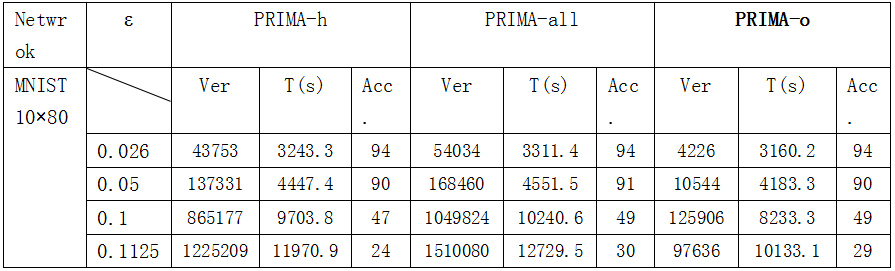
\includegraphics[width=\textwidth]{Fig/FigR3_1.png}
\caption{In the this table, \textit{Ver} is the number of constrains generated by the strategy. \textit{T} is the whole time for the program of the strategy. \textit{Acc.} is the number of verified images among 100 pictures in MNIST test set.} \label{table1}
\end{figure}

According to Fig.~\ref{table1}, on the one hand, we can find that the number of verified images obtained by PRIMA-o is always more than the one obtained by PRIMA-h, and the execution time of ours is always less than  the one of PRIMA-h. The reason is that the heuristic selection strategy of PRIMA-h ignore some points while doing multi-verification in order to save time, the ignored part bring the loss of accuracy. On the other hand, because PRIMA-all consider all of the possible groups to generate constrains, the constrains generated from our strategy are included in it. This experiment prove that our strategy can save a lot of computer sources with losing a little of accuacy through comparing with PRIMA-all. For example, when $\epsilon =0.1125$, PRIMA-o work about 20.3\% faster than PRIMA-all with losing about 3.3\% verified pictures on the 10$\times $80 MNIST network.

%%%%%%%%%%%%%%%%%%%%%%%%%%%%%%%%%%%%%%%%%%%%%%%%%%%%%%%%%%%%%%%%%%%%%%%%%%%%%%%%%%%%%%%%%%%%%%%%%%%%%%

\subsection{Improvement for precision on high-dimensional networks}

In this experiment, we take the first 10 images from test set of MNIST as input. Respectively use PRIMA-all, PRIMA-o, and PRIMA-h to calculate the robust radius of these 10 images on 10$times\ $80 MNIST network in order to comspare the difference on accuracy among these three strategies, under $k=2$. The method of calculating robust radius is dichotomy~\cite{ref_article5} and the iterations is 15, accurating to the extreme position, the result shown by Fig.~\ref{table2}.

\begin{figure}
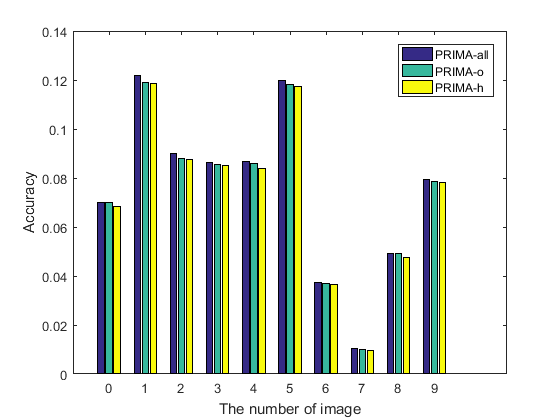
\includegraphics[width=\textwidth]{Fig/FigR3_2.png}
\caption{Comparison of verified robust radius among PRIMA-all, PRIMA-h, and PRIMA-o.} \label{table2}
\end{figure}

In the histogram in Fig~\ref{table2}, the blue part means the robust radius obtained by PRIMA-all, the cyan one means the robust radius obtained by PRIMA-o, the yellow one means the robust radius obtained by PRIMA-h. PRIMA-all cost XXXs to get only about 0.0017 advance than PRIMA-h, however, PRIMA-o just spending XXXs will have about 0.0015 adcanve than PRIMA-h. According to the experiment, PRIMA-o fills the accuracy gap between PRIMA-all and PRIMA-h and cost less time than others.


%%%%%%%%%%%%%%%%%%%%%%%%%%%%%%%%%%%%%%%%%%%%%%%%%%%%%%%%%%%%%%%%%%%%%%%%%%%%%%%%%%%%%%%%%%%%%%%%%%%%%%

\section{Conclusion}
Among the severals of NN verification methods, considering the relationships and constrains among points in the same pre-activation layer is a new and promising direction. It provide a novel and effeciive way to overcome the $Delta$ barrier produced by just considering the constrains of one point. In this paper, according to some experments fact from other work and mathematical theories, we propose a new method and thinking to select which pairs of points is better to generate multi-neuron approximations. The experimental result shows that our method can economize a lot of time and computer resources with losing a little of accuracy under $k=2$.\\
It is worth noticing that our method can be expanded to higher dimensional situation to solve the situation when $k\geq 2$ and can used under sigmoid or tanh instead of ReLU, and these will be the research directions of our team. On the other hand, the most interesting thing is that, although it has work that uses three-dimensional convex hull to do the sybolic propagation, it doesn't expand to higher dimension. It is possible to use the approximations mentioned in our method to achieve multi-neuron propagation with high accuracy and lower time cost in the future.


%%%%%%%%%%%%%%%%%%%%%%%%%%%%%%%%%%%%%%%%%%%%%%%%%%%%%%%%%%%%%%%%%%%%%%%%%%%%%%%%%%%%%%%%%%%%%%%%%%%%%%
\begin{thebibliography}{8}
\bibitem{ref_book1}
G. P. Collins : The shapes of space, Sci. Amer., 291 (2004), pp. 94–103. SCAMAC 0036-8733

\bibitem{ref_url1}
Dimensions:a walk through mathematics, \url{http://www.dimensions-math.org/Dim_ZH_si.htm} Last accessed in
June 2022

\bibitem{ref_article1}
Zhaokui He, Sujuan Zhang, Zhongxi Sun, The Geometric Significance of Determinant and Calculation of Polyhedron Volume. COLLEGE MATHEMATICS \textbf{37}(3), 105--109 (2021)

\bibitem{ref_article2}
Karl Bringmann, Tobias Friedrich, Approximating the volume of unions and intersections
of high-dimensional geometric objects. Computational Geometry \textbf{43}, 601--610 (2010)

\bibitem{ref_article3}
LARRY T. COOK, P. NONG COOK, KYO RAK LEE, SOLOMON BATNITZKY, BERT Y. S. WONG, STEVEN L. FRITZ, JONATHAN OPHIR, SAMUEL J. DWYER III, LAWRENCE R. BIGONGIARI, AND ARCH W. TEMPLETON, An Algorithm for Volume Estimation Based on Polyhedral Approxi mation, IEEE TRANSACTIONS ON BIOMEDICAL ENGINEERING \textbf{27}(9), 493--500 (1980)

\bibitem{ref_url2}
Qhull. "The Geometry Center Home Page." \url{http://www.qhull.org/} Last accessed in
June 2022

\bibitem{ref_article4}
J.B.Lasserre, An Analytical Expression and an Algorithm for the Volume of a Convex Polyhedron in $R^{n}$, JOURNAL OF OPTIMIZATION THEORY AND APPLICATIONS \textbf{39}(3), 363--377 (1983)

\bibitem{ref_url3}
Gurobi Optimization, LLC, "Gurobi optimizer reference manual." \url{http://www.gurobi.com} Last accessed in July 2022

\bibitem{ref_url4}
SRI Lab, ETH Zurich, "eran." \url{https://github.com/eth-sri/eran} Last accessed in July 2022

\bibitem{ref_article5}
Guy Katz, Clark Barrett, David Dill, Kyle Julian and Mykel Kochenderfer, Reluplex: An Efficient SMT Solver for Verifying Deep Neural Networks, CAV (2017)
%%%%%%%%%%%%%%%%%%%%%%%%%%%%%%%%%%%%%%%%%%%%%%%%%%%%%%%%%%%%%%%%%%%%%%%%%%%%%%%%%%%%%%%%%%%%%%%%%%%%%%

%
% the environments 'definition', 'lemma', 'proposition', 'corollary',
% 'remark', and 'example' are defined in the LLNCS documentclass as well.
%
\begin{proof}
Proofs, examples, and remarks have the initial word in italics,
while the following text appears in normal font.
\end{proof}
For citations of references, we prefer the use of square brackets
and consecutive numbers. Citations using labels or the author/year
convention are also acceptable. The following bibliography provides
a sample reference list with entries for journal
articles~\cite{ref_article}, an LNCS chapter~\cite{ref_lncs}, a
book~\cite{ref_book}, proceedings without editors~\cite{ref_proc},
and a homepage~\cite{ref_url}. Multiple citations are grouped
\cite{ref_article,ref_lncs,ref_book},
\cite{ref_article,ref_book,ref_proc1,ref_url}.
%
% ---- Bibliography ----
%
% BibTeX users should specify bibliography style 'splncs04'.
% References will then be sorted and formatted in the correct style.
%
% \bibliographystyle{splncs04}
% \bibliography{mybibliography}
%

\bibitem{ref_article}
Author, F.: Article title. Journal \textbf{2}(5), 99--110 (2016)

\bibitem{ref_lncs}
Author, F., Author, S.: Title of a proceedings paper. In: Editor,
F., Editor, S. (eds.) CONFERENCE 2016, LNCS, vol. 9999, pp. 1--13.
Springer, Heidelberg (2016). \doi{10.10007/1234567890}

\bibitem{ref_book}
Author, F., Author, S., Author, T.: Book title. 2nd edn. Publisher,
Location (1999) pp. 94–103. SCAMAC 0036-8733

\bibitem{ref_proc}
Author, A.-B.: Contribution title. In: 9th International Proceedings
on Proceedings, pp. 1--2. Publisher, Location (2010)

\bibitem{ref_url}
LNCS Homepage, \url{http://www.springer.com/lncs}. Last accessed 4
Oct 2017
\end{thebibliography}
\end{document}
